\chapter{绪论}

\section{课题背景及意义}
绿色能源已成为当今世界能源发展的主要趋势。未来人类可能会面对全球能源危机,发展绿色能源是能源发展惟一的出路。
各国政府纷纷制定了本国的绿色能源发展计划。在港口码头领域,绿色能源,清洁能源正发挥着越来越重要的作用。

船舶停靠码头时,装卸货物电气设备所需电力主要是从船舶电力系统来获取。船舶靠岸期间,用电是由船上的辅机组提供,
辅机发电会消耗化石燃料,主要是重油或者柴油。发电机组工作过程中,化石燃料的使用会排放诸如氮氧化合物,硫氧化合物,
和粉尘等一些污染物,会对港口空气质量造成一定的影响,同时发电机组会产生较大的噪声,影响港口附近人员的工作和
生活。

为了建立绿色港口,清洁港口,减少污染物的排放,船舶在停靠港口时,可以停止使用用柴油发电机组发电,
改用岸上电力系统提供所需电力。中国是世界上最大的航运国家,2020年,全球前20大集装箱港口中国仍占近半数,前10
大集装箱港口中有7个来自中国,中国港口货物吞吐量连年增长。根据国际海事组织(IMO)研究数据表明,2020年,全球
航运业需要4亿吨燃料,排放14亿吨$CO_{2}$,约占全球$CO_{2}$总排放量的$6\%$。保守的估计,我国每年靠港船舶
消耗的燃料油约为$70$万吨,船舶辅机发电的碳排量占港口总碳排量的40\%\~{}70\%\cite{SP1}。

岸电在美国西海岸已是强制性要求,在我国和一些亚洲国家尚在发展之中。我国交通部颁布的《船舶与港口污染防治专项行动实施方案》
(2015-2020年)对促进岸电发展发挥了巨大作用,截至2020年我国$90\%$的公务船舶、港作船舶靠泊时使用了岸电,
$50\%$的客滚、集装箱和邮轮专业化码头具有向船舶提供岸电的能力。港口应用岸电后,船舶靠港时污染物的排放
明显减少,港口环境得到了改善。应用船岸连接技术,对于港口地区的环境保护有重大的意义,
如果船舶岸电技术得到大力发展,所有靠港船舶都由岸电提供电力,那么既可以降低$30\%$的燃油成本\cite{SP2}和节省部分的维护成本,
也能够帮助港口满足IMO减排目标,为国家绿色可持续发展助力。

国家十四五规划,对碳排放,空气污染物的排放量对作出了约束性的规定,
推广使用岸电技术是保护港口环境,减排防污的一大重要举措,对建设生态文明友好型的港口具有重大意义。
表\ref{tab:岸电替代效益}中数据显示,船舶靠港使用岸电后,微尘等颗粒物的排放减少了78\%,空气污染物$SO_{x}$、
$NO_{x}$的每$KWh$排放量分别减少了74\%和80.1\%,环境保护与改善的效果明显。

\begin{table}[!htp]
	\centering
	\caption[中国岸电替代辅机发电的减排表现]{中国岸电替代辅机发电的减排表现\cite{SP3}}
	\label{tab:岸电替代效益}
	\resizebox{\textwidth}{!}{%
	\begin{tabular}{c}
		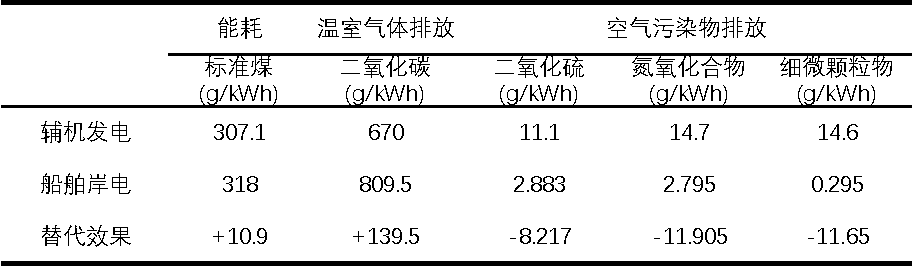
\includegraphics{岸电替代效益.pdf} 
	\end{tabular}
	}
\end{table}

电气化,自动化,智能化是全球大趋势,工业过程、城市交通、供热和制冷在未来将由从$CO_{2}$零排放的
绿色可再生能源获得的电力来供电。到 2050年,全球发电容量预计将达到当前发电容量的两倍或三倍,
岸电是我国在交通领域实现电气化的重要部分。

总之,船舶靠港停用辅机改用岸电是港口码头实现防污减排的首选方案,这在全球范围内取得了一定的共识。
其次,船舶辅机的发电效率并不是很高,改用岸电后,接入电网按时计价,具有良好的替代经济效益。
最后,发展岸电技术,提高港口自动化率,是中国制造的内在要求。未来,伴随着一带一路的发展,沿线国家的港口势必
会迎来更多的中国货船,推广中国岸电的技术,制定中国标准显得十分必要。
中国在成为科技强国的路上,必须大力发展先进技术,在港口领域,我们要大力发展电气化,自动化和智能化的港口,
具体到电气化,则需要大力推广船舶岸电技术,推动船岸连接系统的完善。


\section{船岸连接系统研究现状}
目前,受港口空气污染的压力,国内外均对船舶岸电系统进行了研宄和设计。欧美国家的一些港口己经大规模地
对靠港船舶进行供电,港区污染气体排放明显减少,港口的空气质量得到有效的改善。对于船舶岸电系统相关
标准的制定也逐渐趋于完善。相对于国外,国内对船舶岸电系统的研究起步较晚,虽然全国范围内港口岸电系统
改造遍地开花,但仍处于试验阶段,推广工作任重而道远。


\begin{figure}[!htp]
	\centering
	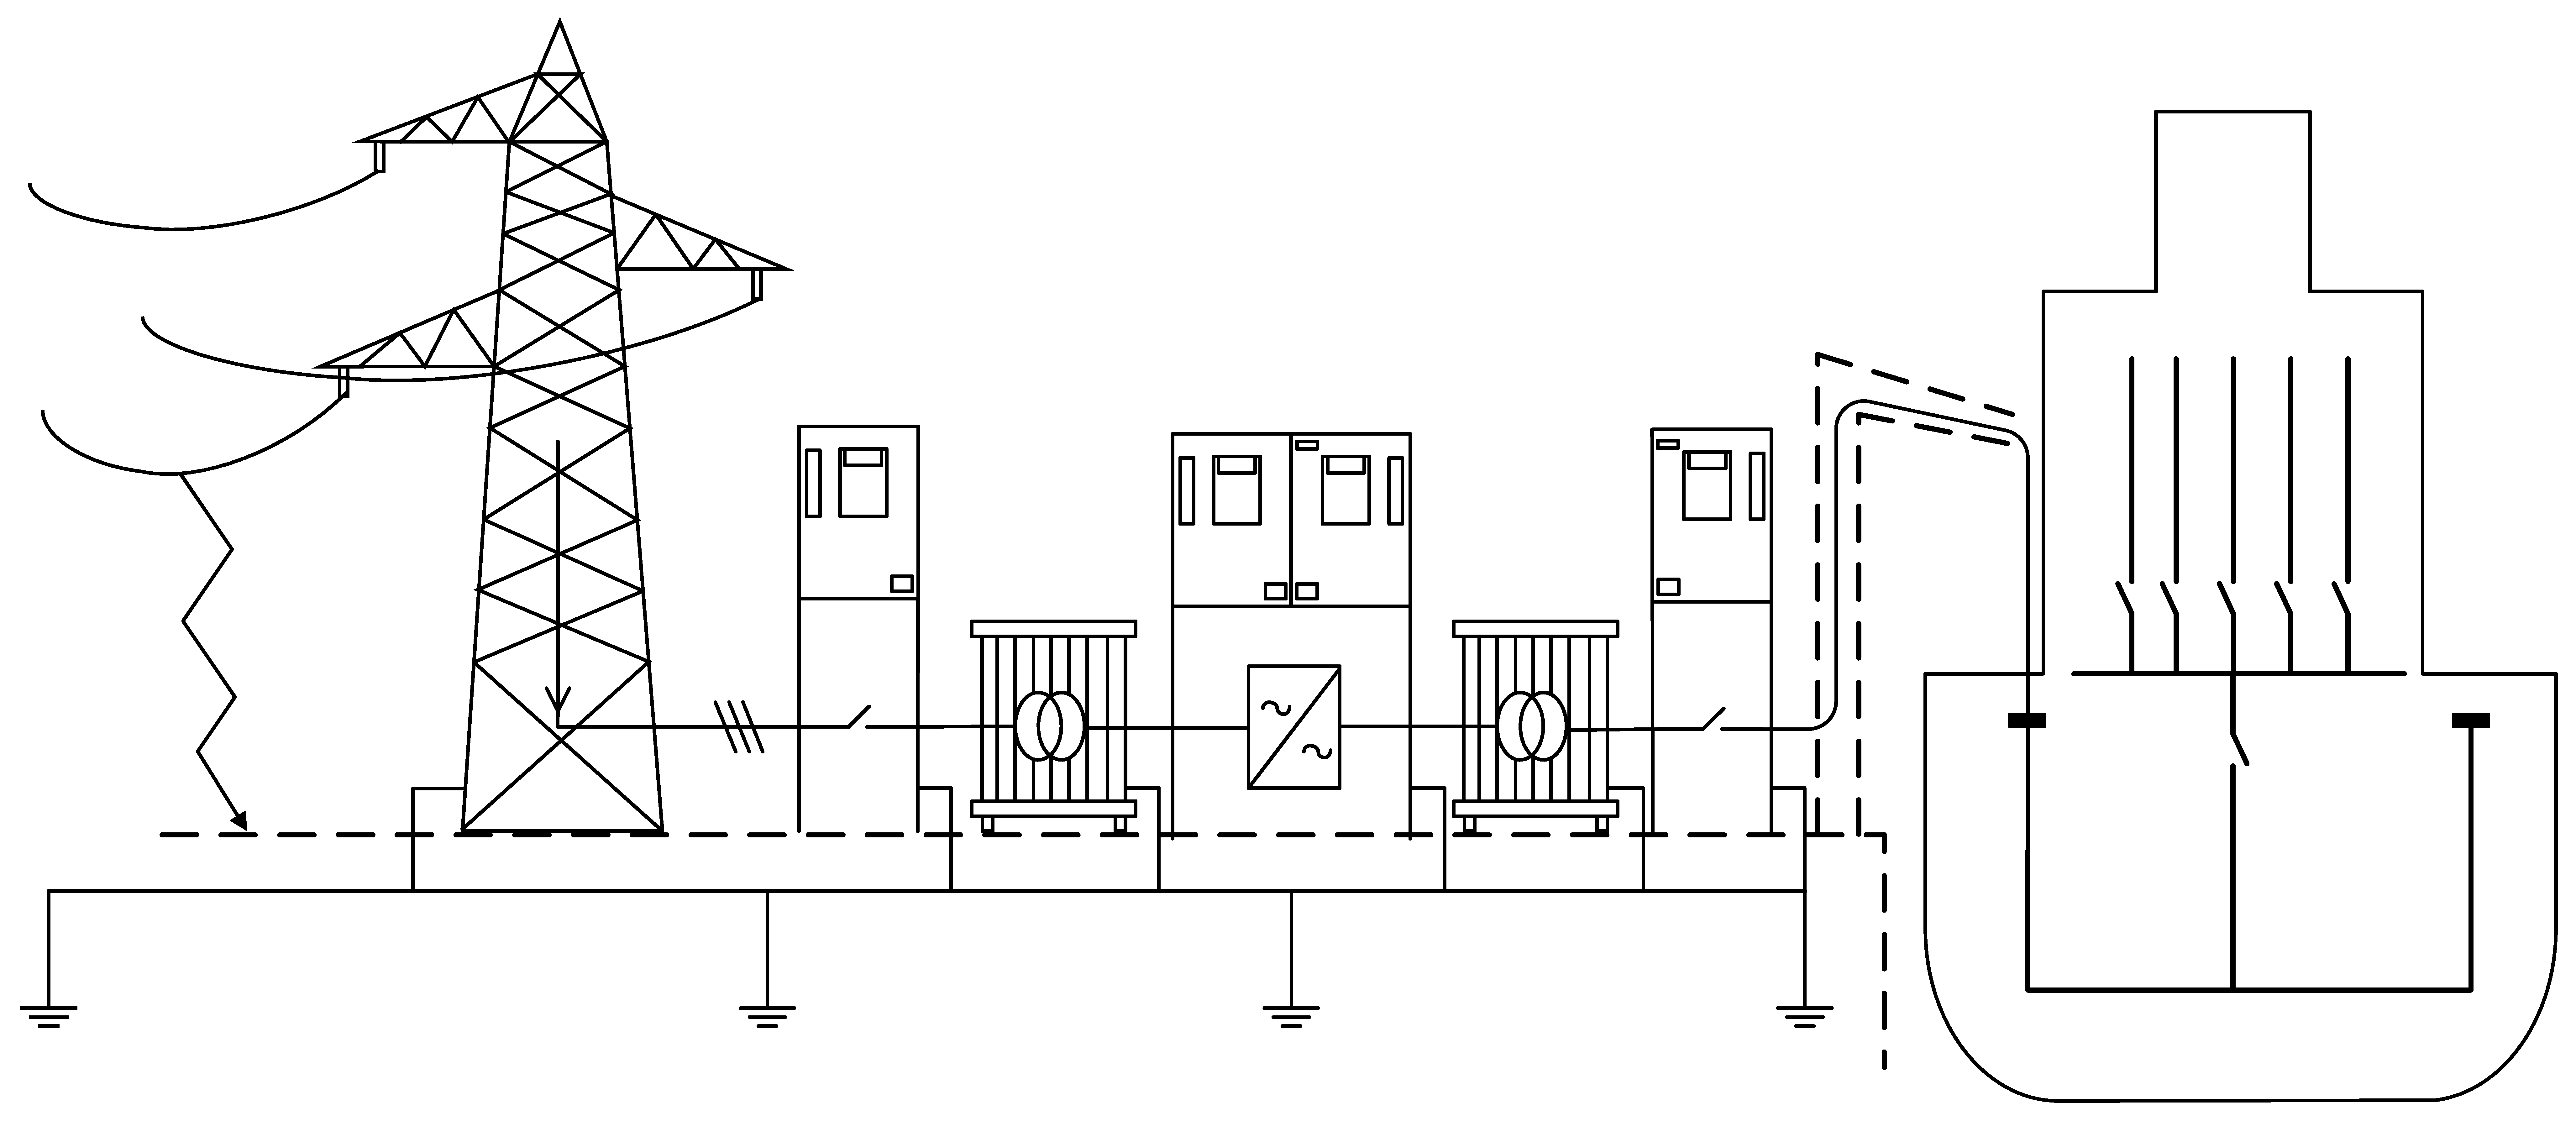
\includegraphics[width=0.95\textwidth]{高压船岸连接示意图.pdf}
	\caption{船岸连接示意图}
	\label{fig:船岸连接示意图}
\end{figure}



岸电(SP),文献中也有不同名称的称呼,如冷熨烫、船岸连接、岸电(SSE)、岸电供电、岸电供电(OPS)、替代海电(AMP) 
(Arduino和Carrillo Murillo,2011;Kalikatzarakis等人,2018年;陈等,2019;Kumar等人,2019年;彭等,2019),
涉及停泊船舶关闭其船载辅助发动机,并使用港口提供的清洁能源为船载主要系统供电,并满足所有船载设施的电力需求,
如照明、制冷和货物卸载设施。这种技术允许停泊的船只使用SP,而不是依靠辅助发动机产生的动力来减少港口的废气排放(Ballini和Bozzo,2015年)。
它需要三个基本组件:岸侧电气系统和基础设施、电缆管理系统和船侧电气系统(Tseng and Pilcher,2015),如图1所示。
岸侧电气系统将高压变电站的电力传输到船舶附近的连接点,即终端的配电箱,以转换电压电平、转换频率、
以不间断的方式在船舶电力接收系统之间切换等。电缆管理系统包括连接岸侧连接点和船载受电设施的电缆和设施。
电缆连接设施必须满足快速连接和储存的要求,不使用时应存放在船上、岸上或驳船上。船侧电气系统是在原有船载配电
系统基础上增加的受电单元,包括电缆绞车、变压器及相关管理系统(陈等,2019)。船载电站的发电机按电压等级可分为
高压和低压。高压船载电站的电压等级包括11 kV、6.6 kV (60 Hz)和6 kV (50 Hz),低压船载电站的电压等级包括400 V (50 Hz)
和440伏(60赫兹)(Tian等人,2014年)

随着近年来全球货运量和客运量的增加,航运预计将成为增长最快的温室气体排放者之一(Styhre等人,2017年)。
其中,使用辅助发动机发电的停泊船舶造成的空气和噪声污染日益成为影响沿海港口城市环境的重要问题。
早在2000年,瑞典哥德堡港就设计并安装了世界上第一个高压SP系统,该系统将停泊船舶的污染物排放量减少了94\%-97\%(陈等人,2019年)。
2001年,美国港使用SP系统向五艘改装的游轮供电,标志着SP技术首次应用于豪华游轮码头(田等人,2014年)。
SP系统在欧盟和美国引起了广泛关注。2004年,美国洛杉矶港首次将SP应用于集装箱码头,并计划于2014年在所有集装箱码头
安装SP设施。2009年,长滩港首次将该系统应用于石油码头。2012年后,在纽约布鲁克林邮轮码头、安特卫普港集装箱码头、
吕贝克港等也安装了SP供应系统。




\subsection{国外应用状况}


\begin{figure}[!htp]
	\centering
	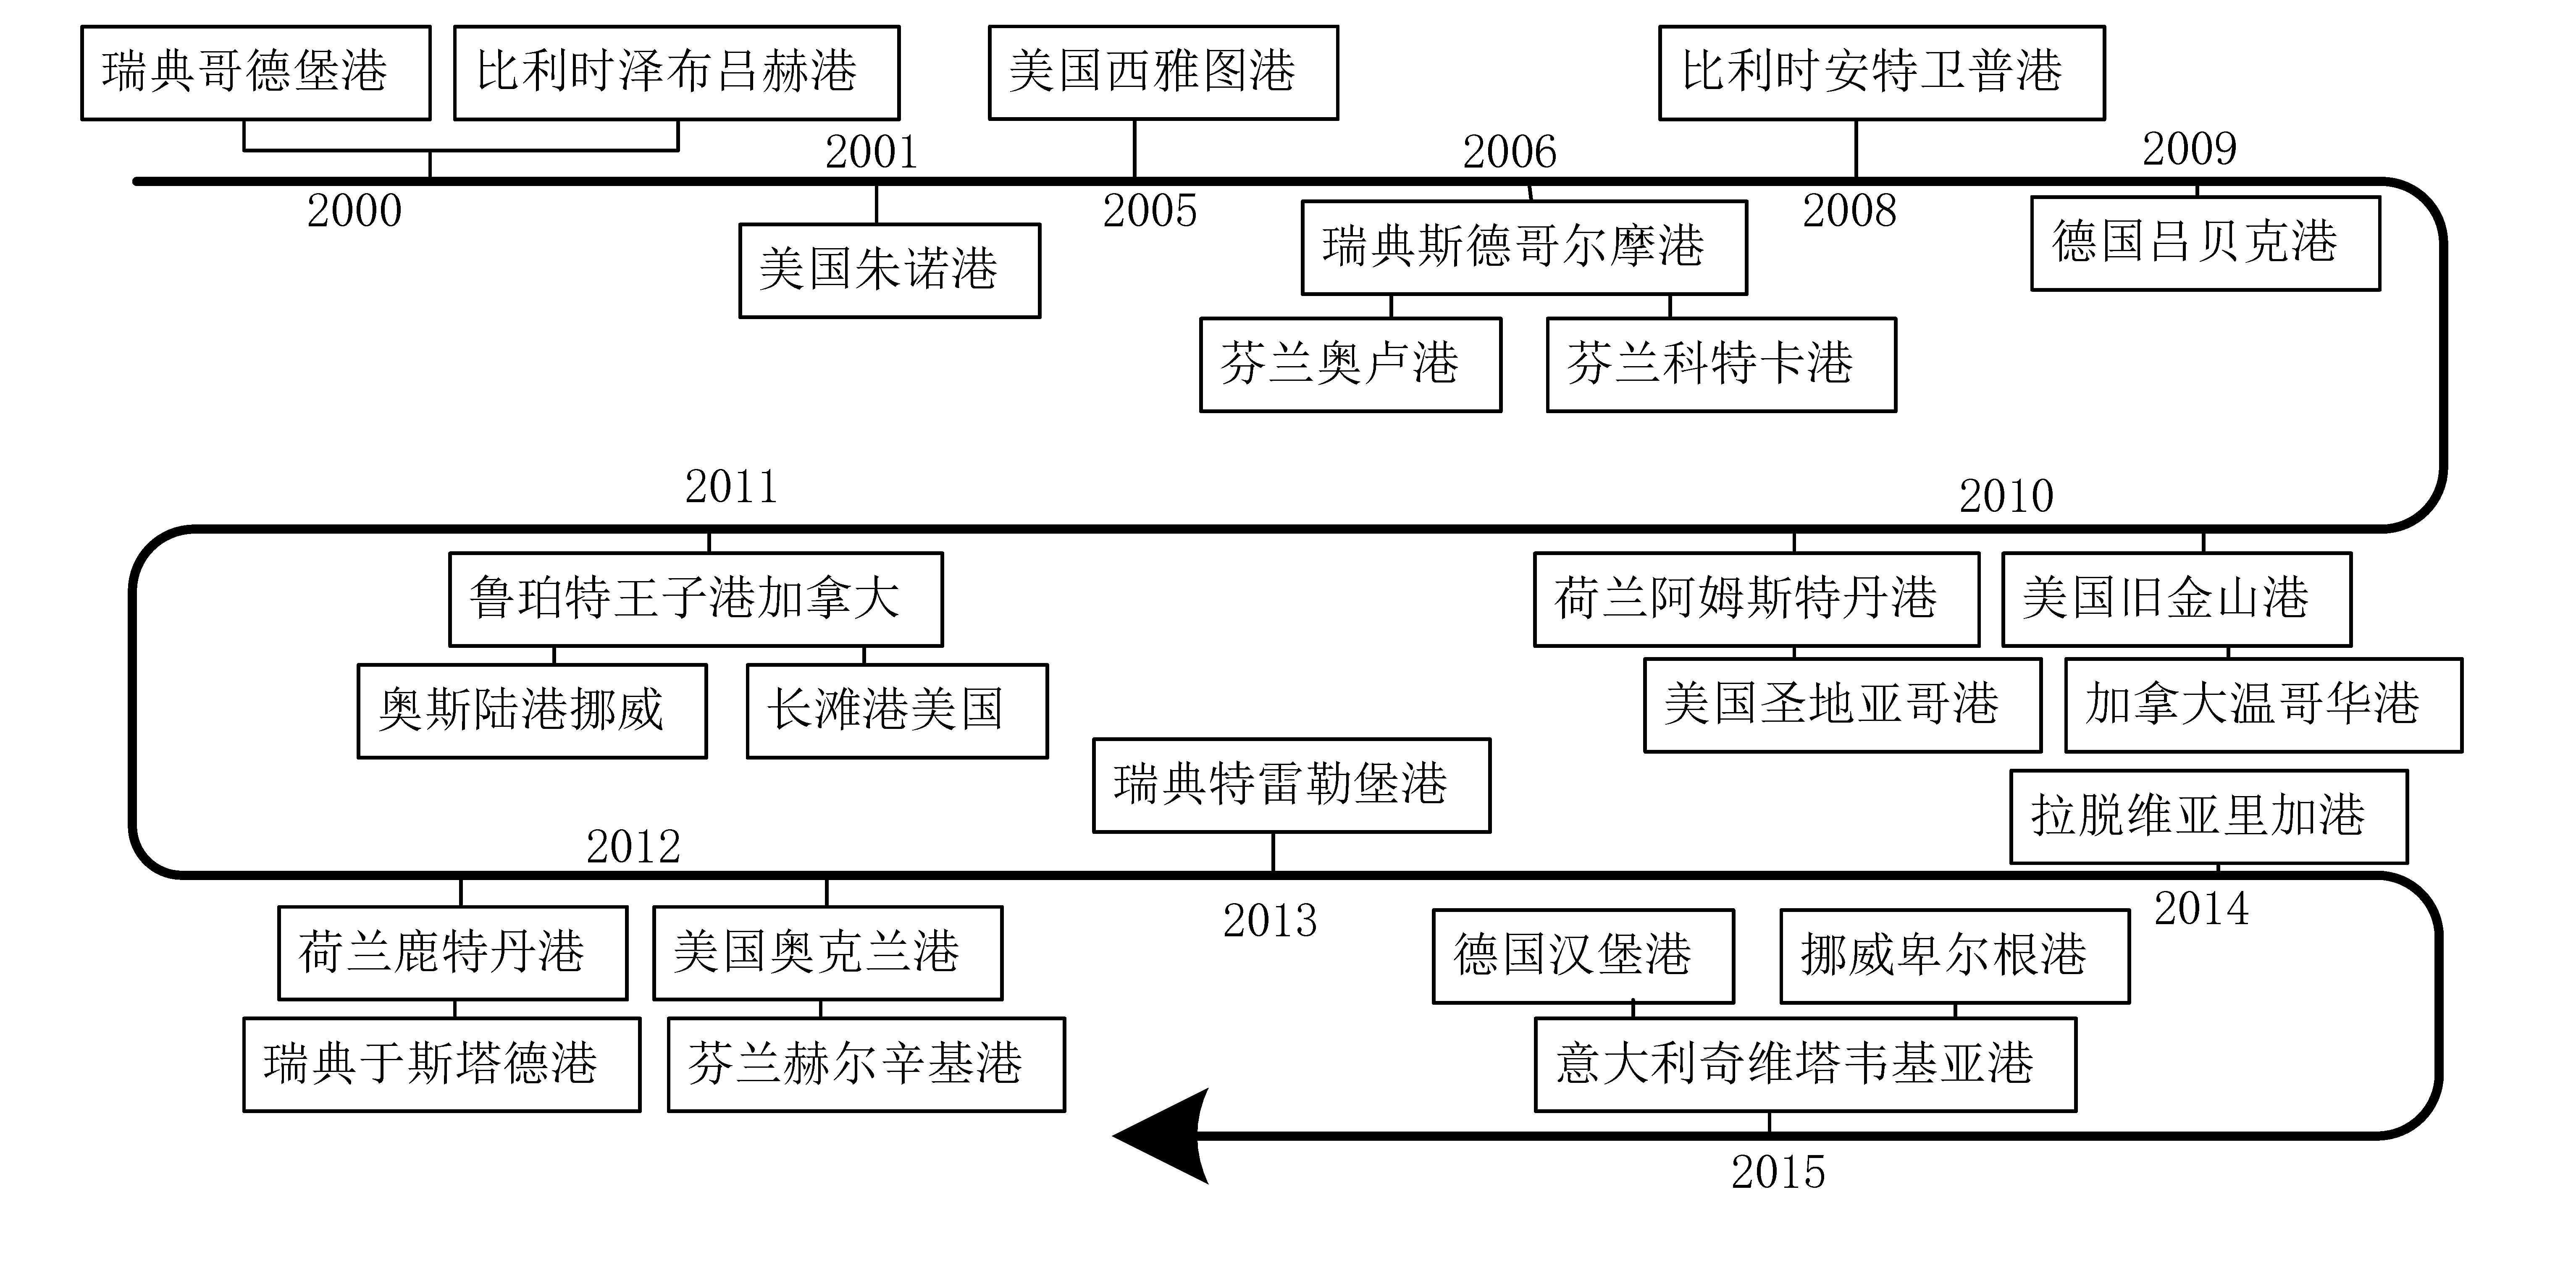
\includegraphics[width=0.9\textwidth]{国外应用岸电技术的主要港口.pdf}
	\caption{国外主要港口的岸电发展}
	\label{fig:国外主要港口的岸电发展}
\end{figure}


\zhlipsum[6]
\subsection{国内应用状况}


\begin{figure}[!htp]
	\centering
	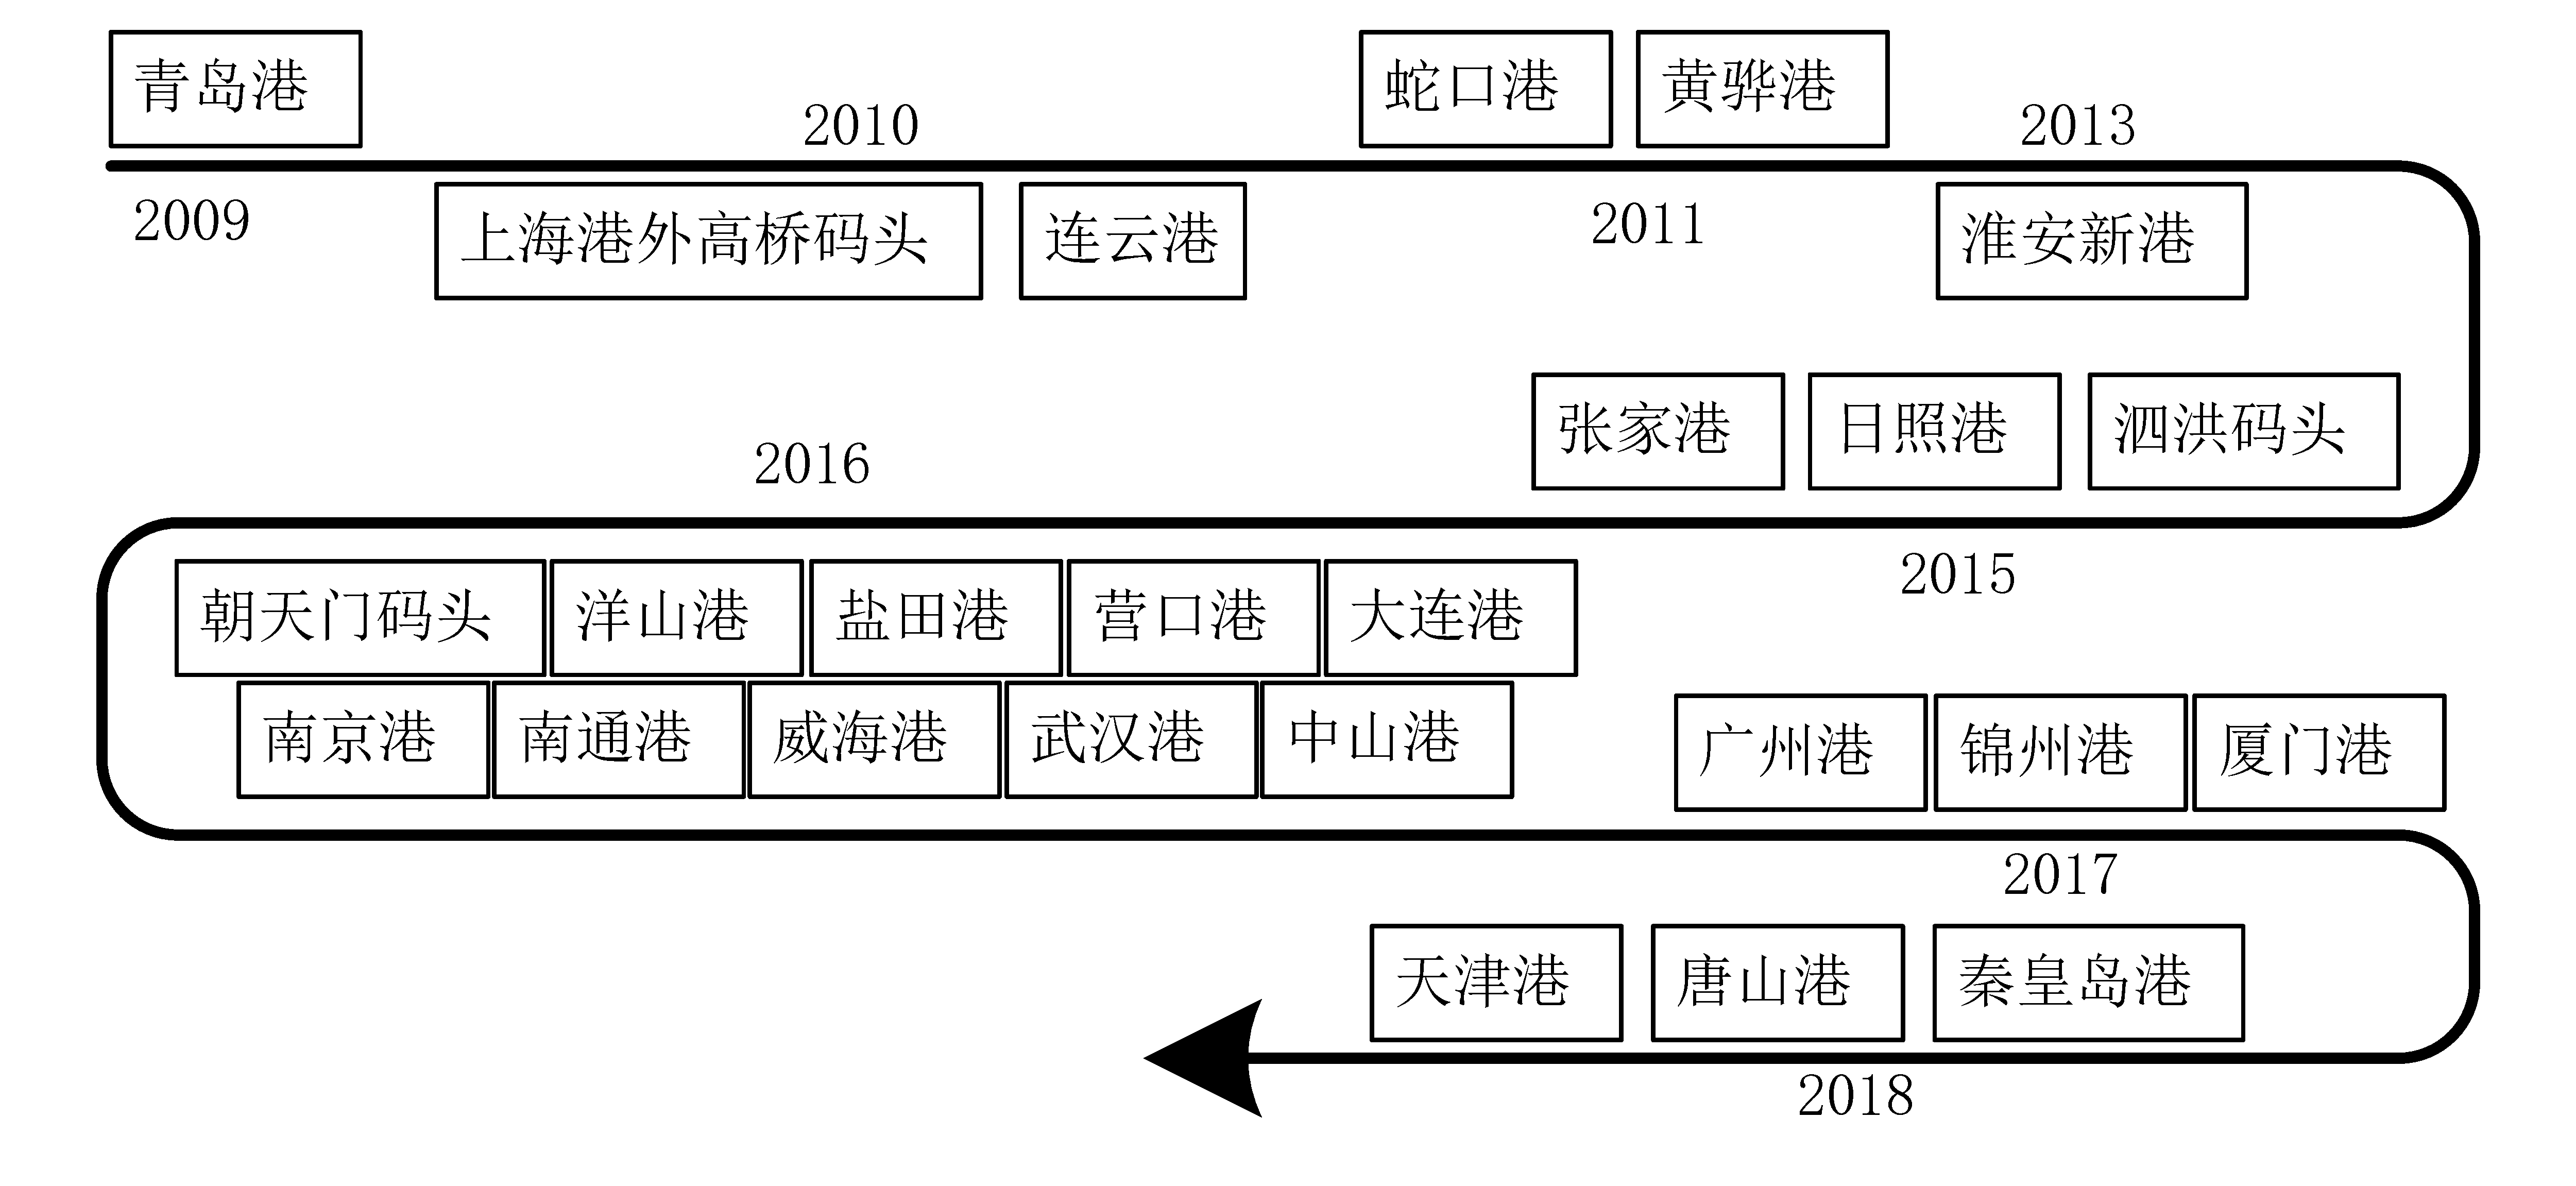
\includegraphics[width=0.85\textwidth]{国内应用岸电技术的主要港口.pdf}
	\caption{国内主要港口的岸电发展}
	\label{fig:国内主要港口的岸电发展}
\end{figure}




\zhlipsum[7]

\begin{figure}[!htp]
	\centering
	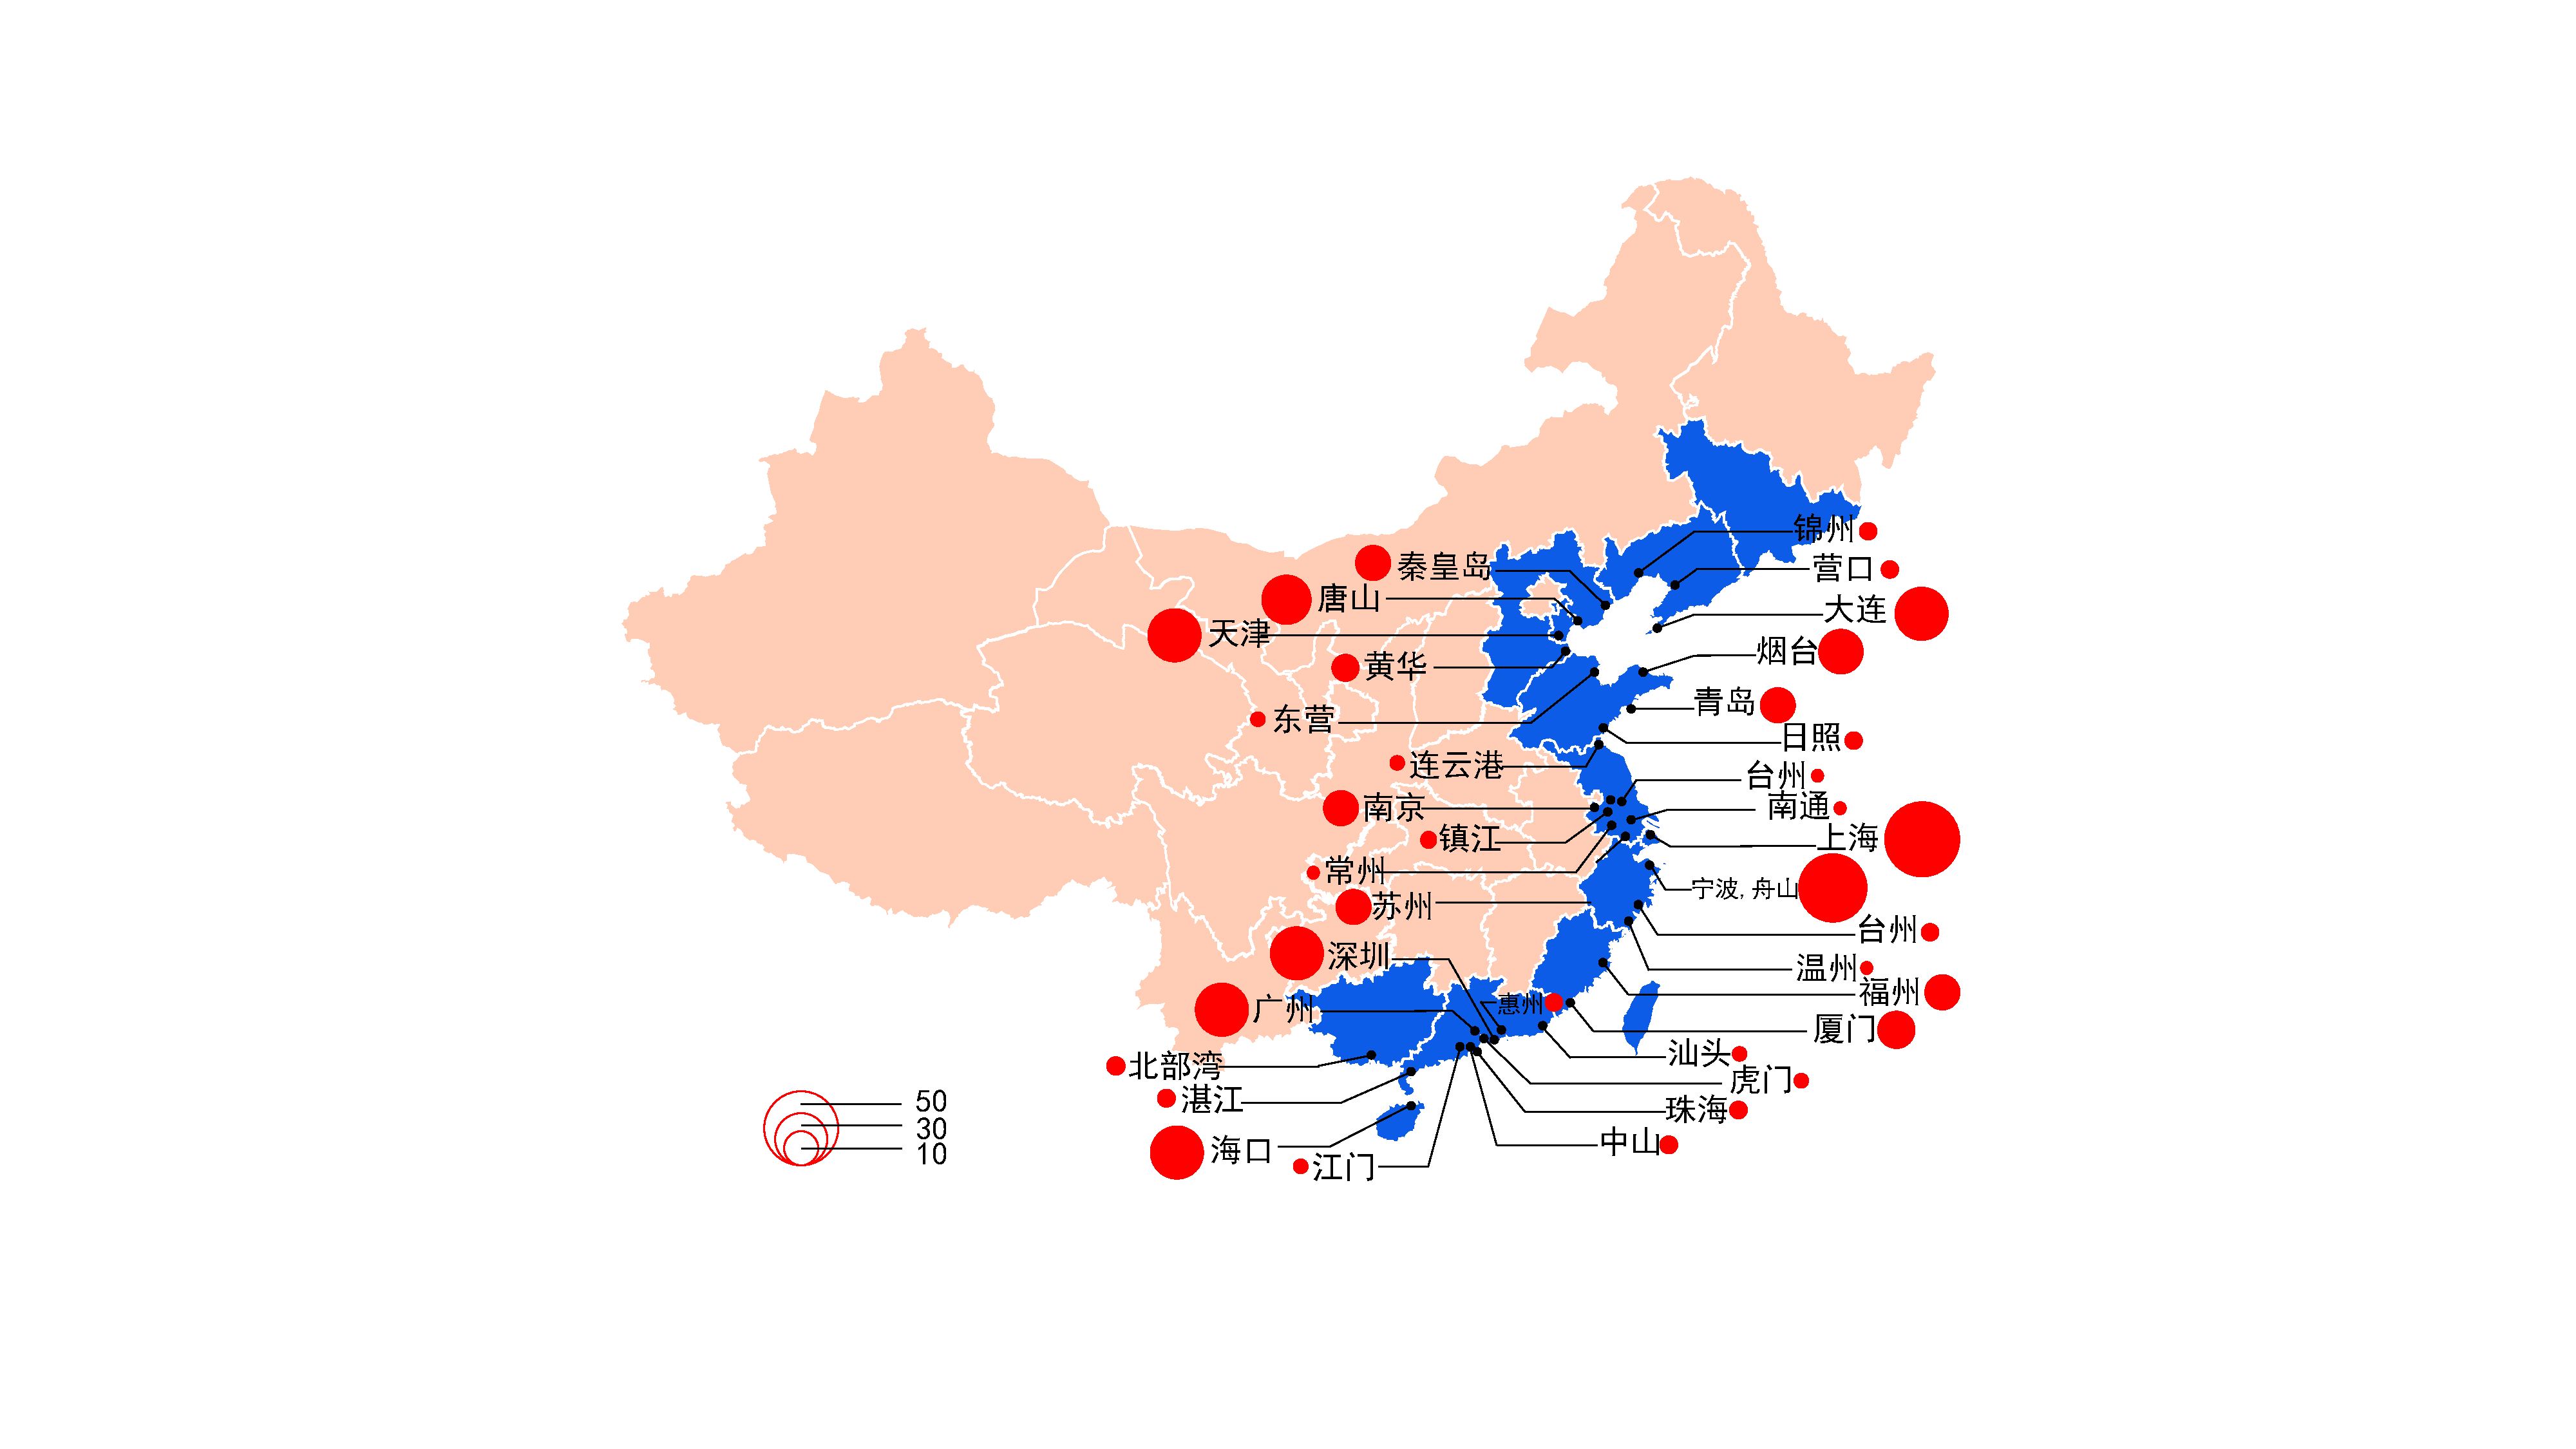
\includegraphics[width=0.9\textwidth]{中国岸电分布图.pdf}
	\caption{中国岸电分布图}
	\label{fig:中国船电分布图}
\end{figure}

\section{论文研究内容及工作}
\zhlipsum[8]
